\documentclass{article}
\usepackage[utf8]{inputenc}
\usepackage[T1]{fontenc}

% Set page geometry
\usepackage[margin=2.5cm,headsep=0.5cm]{geometry}

% AMS and mathtools
\usepackage{amsmath,amsthm,amssymb,marvosym,mathrsfs,amsfonts,amscd,mathtools}

% Hyperlinks and URLs
\usepackage{url}
\usepackage{hyperref}
\hypersetup{
    colorlinks,
    citecolor=BLACK,
    filecolor=BLACK,
    linkcolor=BLACK,
    urlcolor=BLACK
}

% Colors
\usepackage{xcolor}

% Bold math
\usepackage{bm}

% Bra Ket (Dirac) Notation
\usepackage{braket}

% Slashed characters (e.g. in Dirac equation)
\usepackage{slashed}

% Clean SI Units
\usepackage{siunitx}

% Enumerate thingies
\usepackage{enumitem}

% Cancel things out in equations
\usepackage[makeroom]{cancel}

% Graphics and figures
\usepackage{graphicx}
\usepackage{wrapfig}
\usepackage{float}

% Caption figures and tables
\usepackage{caption,subcaption}

% Generate symbols
\usepackage{textcomp} % Include this line to avoid output errors
\usepackage{gensymb}

% Make multiple rows in a table
\usepackage{multirow}

% Booktabs tables
\usepackage{booktabs}

% Useful frames
\usepackage{mdframed}

% Comment-out large sections
\usepackage{comment}

% No auto-indent
\setlength{\parindent}{0pt}

% Asymptote - 3D vector graphics
\usepackage{asymptote}

% Tikz Package Stuff
\usepackage{pgf,tikz,pgfplots}
\usepackage{tikz-3dplot}
% Use various tikz libraries
\usetikzlibrary{decorations.pathmorphing, decorations.markings, decorations.pathreplacing, patterns} % Decorate paths!
\usetikzlibrary{calc}
\usetikzlibrary{scopes}
\usetikzlibrary{angles, quotes}
\usetikzlibrary{svg.path}
\usetikzlibrary{arrows, arrows.meta}
\usetikzlibrary{fadings}
% pgfplots package settings
\pgfplotsset{compat=1.15}
% \pgfplotsset{width=10cm,compat=1.9} % Taken from latest overleaf.


% Awesome circled numbers
\newcommand*\circled[4]{\tikz[baseline=(char.base)]{\node[shape=circle, fill=#2, draw=#3, text=#4, inner sep=2pt] (char) {#1};}}

% Control size of text
\usepackage{relsize}

% Extend conditional commands
\usepackage{xifthen}

% Scale math by size
\newcommand*{\Scale}[2][4]{\scalebox{#1}{\ensuremath{#2}}}

% Big integrals
\usepackage{bigints}

% Number equations within sections
\numberwithin{equation}{section}

% Generate blind text
\usepackage{blindtext}

% Useful symbols
\usepackage{marvosym}


%%%% THEOREMS %%%%
\newenvironment{theorem}[1][\hspace{-0.36em}]
{
    \begin{mdframed}[backgroundcolor=black!4, align=center, userdefinedwidth=40em, topline=false, bottomline = false, leftline = false, rightline = false, frametitle = {#1 Theorem}]
}
{
    \end{mdframed}
}

%%%% LEMMAS %%%%
\newenvironment{lemma}[1][\hspace{-0.36em}]
{
    \begin{mdframed}[backgroundcolor=black!4, align=center, userdefinedwidth=40em, topline=false, bottomline = false, leftline = false, rightline = false, frametitle = {#1 Lemma}]
}
{
    \end{mdframed}
}

%%%% COROLLARY %%%%
\newenvironment{corollary}[1][\hspace{-0.36em}]
{
    \begin{mdframed}[backgroundcolor=black!4, align=center, userdefinedwidth=40em, topline=false, bottomline = false, leftline = false, rightline = false, frametitle = {#1 Corollary}]
}
{
    \end{mdframed}
}

%%%% DEFINITIONS %%%%
\newenvironment{definition}[1][\hspace{-0.36em}]
{
    \begin{mdframed}[backgroundcolor=black!4, align=center, userdefinedwidth=40em, topline=false, bottomline = false, leftline = false, rightline = false, frametitle = {#1 Definition}]
}
{
    \end{mdframed}
}

%%%% PROPOSITION %%%%
\newenvironment{proposition}
{
    \begin{mdframed}[backgroundcolor=black!4, align=center, userdefinedwidth=40em, topline=false, bottomline = false, leftline = false, rightline = false, frametitle = {Proposition}]
}
{
    \end{mdframed}
}

% Change end-of-proof symbol
\renewcommand\qedsymbol{$\blacksquare$}


%%%% BLACKBOARD BOLD %%%%
\newcommand{\bbN}{\mathbb{N}} % Natural numbers
\newcommand{\bbZ}{\mathbb{Z}} % Zahlen
\newcommand{\bbQ}{\mathbb{Q}} % Rational numbers
\newcommand{\bbR}{\mathbb{R}} % Real numbers
\newcommand{\bbC}{\mathbb{C}} % Complex numbers
\DeclareSymbolFont{bbold}{U}{bbold}{m}{n} % Identity matrix
\DeclareSymbolFontAlphabet{\mathbbold}{bbold} % Identity matrix
\newcommand{\identitymatrix}{\mathbbold{1}} % Identity matrix


%%%% CODE LISTING %%%%
\usepackage{listings}
\definecolor{greencomments}{HTML}{00BA00}
\definecolor{graynumbers}{HTML}{4F4F4F}
\definecolor{purplestrings}{HTML}{AD00AA}
\definecolor{backgroundcolor}{HTML}{E8E8E8}
\lstdefinestyle{nkostin}{
    backgroundcolor=\color{backgroundcolor},   
    commentstyle=\color{greencomments},
    keywordstyle=\color{blue},
    numberstyle=\tiny\color{graynumbers},
    stringstyle=\color{purplestrings},
    basicstyle=\footnotesize,
    breakatwhitespace=false,         
    breaklines=true,                 
    captionpos=b,                    
    keepspaces=true,                 
    numbers=left,                    
    numbersep=5pt,                  
    showspaces=false,                
    showstringspaces=false,
    showtabs=false,                  
    tabsize=2
}
\lstset{style=nkostin}

%%%% UNIT BASIS VECTORS %%%%
\newcommand{\ihat}{\bm{\hat{\imath}}} % Cartesian i hat (x-direction)
\newcommand{\jhat}{\bm{\hat{\jmath}}} % Cartesian j hat (y-direction)
\newcommand{\khat}{\bm{\hat{k}}} % Cartesian k hat (z-direction)
\newcommand{\rhat}{\bm{\hat{r}}} % Spherical r hat
\newcommand{\phihat}{\bm{\hat{\phi}}} % Spherical phi hat
\newcommand{\thetahat}{\bm{\hat{\theta}}} % Spherical theta hat
\newcommand{\nhat}{\bm{\hat{n}}} % Unit normal vector
\newcommand{\rhohat}{\bm{\hat{\rho}}} % Cylindrical rho hat
\newcommand{\zhat}{\bm{\hat{z}}} % Cylindrical z hat


%%%% COLORS: DEFINITIONS AND COMMANDS %%%%
% Miscellaneous
\definecolor{DARKBLUE}{HTML}{040080}
\definecolor{DARKBROWN}{HTML}{8B4513}
\definecolor{LIGHTBROWN}{HTML}{CD853F}
\definecolor{PINK}{HTML}{D147BD}
\definecolor{LIGHTPINK}{HTML}{DC75CD}
\definecolor{GREENSCREEN}{HTML}{00FF00}
\definecolor{ORANGE}{HTML}{FF862F}
\newcommand{\DARKBLUE}{\color{DARKBLUE}}
\newcommand{\DARKBROWN}{\color{DARKBROWN}}
\newcommand{\LIGHTBROWN}{\color{LIGHTBROWN}}
\newcommand{\PINK}{\color{PINK}}
\newcommand{\LIGHTPINK}{\color{LIGHTPINK}}
\newcommand{\GREENSCREEN}{\color{GREENSCREEN}}
\newcommand{\ORANGE}{\color{ORANGE}}
% Blue
\definecolor{BLUEE}{HTML}{1C758A}
\definecolor{BLUED}{HTML}{29ABCA}
\definecolor{BLUEC}{HTML}{58C4DD}
\definecolor{BLUEB}{HTML}{9CDCEB}
\definecolor{BLUEA}{HTML}{C7E9F1}
\definecolor{BLUE}{HTML}{0000FF}
\newcommand{\BLUEE}{\color{BLUEE}}
\newcommand{\BLUED}{\color{BLUED}}
\newcommand{\BLUEC}{\color{BLUEC}}
\newcommand{\BLUEB}{\color{BLUEB}}
\newcommand{\BLUEA}{\color{BLUEA}}
\newcommand{\BLUE}{\color{BLUE}}
% Teal
\definecolor{TEALE}{HTML}{49A88F}
\definecolor{TEALD}{HTML}{55C1A7}
\definecolor{TEALC}{HTML}{5CD0B3}
\definecolor{TEALB}{HTML}{76DDC0}
\definecolor{TEALA}{HTML}{ACEAD7}
\definecolor{TEAL}{HTML}{00FFFF}
\newcommand{\TEALE}{\color{TEALE}}
\newcommand{\TEALD}{\color{TEALD}}
\newcommand{\TEALC}{\color{TEALC}}
\newcommand{\TEALB}{\color{TEALB}}
\newcommand{\TEALA}{\color{TEALA}}
\newcommand{\TEAL}{\color{TEAL}}
% Green
\definecolor{GREENE}{HTML}{699C52}
\definecolor{GREEND}{HTML}{77B05D}
\definecolor{GREENC}{HTML}{83C167}
\definecolor{GREENB}{HTML}{A6CF8C}
\definecolor{GREENA}{HTML}{C9E2AE}
\definecolor{GREEN}{HTML}{00FF00}
\newcommand{\GREENE}{\color{GREENE}}
\newcommand{\GREEND}{\color{GREEND}}
\newcommand{\GREENC}{\color{GREENC}}
\newcommand{\GREENB}{\color{GREENB}}
\newcommand{\GREENA}{\color{GREENA}}
\newcommand{\GREEN}{\color{GREEN}}
% Yellow
\definecolor{YELLOWE}{HTML}{E8C11C}
\definecolor{YELLOWD}{HTML}{F4D345}
\definecolor{YELLOWC}{HTML}{FFFF00}
\definecolor{YELLOWB}{HTML}{FFEA94}
\definecolor{YELLOWA}{HTML}{FFF1B6}
\definecolor{YELLOW}{HTML}{FFFF00}
\newcommand{\YELLOWE}{\color{YELLOWE}}
\newcommand{\YELLOWD}{\color{YELLOWD}}
\newcommand{\YELLOWC}{\color{YELLOWC}}
\newcommand{\YELLOWB}{\color{YELLOWB}}
\newcommand{\YELLOWA}{\color{YELLOWA}}
\newcommand{\YELLOW}{\color{YELLOW}}
% Gold leader standing by
\definecolor{GOLDE}{HTML}{C78D46}
\definecolor{GOLDD}{HTML}{E1A158}
\definecolor{GOLDC}{HTML}{F0AC5F}
\definecolor{GOLDB}{HTML}{F9B775}
\definecolor{GOLDA}{HTML}{F7C797}
\newcommand{\GOLDE}{\color{GOLDE}}
\newcommand{\GOLDD}{\color{GOLDD}}
\newcommand{\GOLDC}{\color{GOLDC}}
\newcommand{\GOLDB}{\color{GOLDB}}
\newcommand{\GOLDA}{\color{GOLDA}}
% Red leader standing by
\definecolor{REDE}{HTML}{CF5044}
\definecolor{REDD}{HTML}{E65A4C}
\definecolor{REDC}{HTML}{FC6255}
\definecolor{REDB}{HTML}{FF8080}
\definecolor{REDA}{HTML}{F7A1A3}
\definecolor{RED}{HTML}{FF0000}
\newcommand{\REDE}{\color{REDE}}
\newcommand{\REDD}{\color{REDD}}
\newcommand{\REDC}{\color{REDC}}
\newcommand{\REDB}{\color{REDB}}
\newcommand{\REDA}{\color{REDA}}
\newcommand{\RED}{\color{RED}}
% Maroon
\definecolor{MAROONE}{HTML}{94424F}
\definecolor{MAROOND}{HTML}{A24D61}
\definecolor{MAROONC}{HTML}{C55F73}
\definecolor{MAROONB}{HTML}{EC92AB}
\definecolor{MAROONA}{HTML}{ECABC1}
\newcommand{\MAROONE}{\color{MAROONE}}
\newcommand{\MAROOND}{\color{MAROOND}}
\newcommand{\MAROONC}{\color{MAROONC}}
\newcommand{\MAROONB}{\color{MAROONB}}
\newcommand{\MAROONA}{\color{MAROONA}}
% Purple
\definecolor{PURPLEE}{HTML}{644172}
\definecolor{PURPLED}{HTML}{715582}
\definecolor{PURPLEC}{HTML}{9A72AC}
\definecolor{PURPLEB}{HTML}{B189C6}
\definecolor{PURPLEA}{HTML}{CAA3E8}
\definecolor{PURPLE}{HTML}{FF00FF}
\newcommand{\PURPLEE}{\color{PURPLEE}}
\newcommand{\PURPLED}{\color{PURPLED}}
\newcommand{\PURPLEC}{\color{PURPLEC}}
\newcommand{\PURPLEB}{\color{PURPLEB}}
\newcommand{\PURPLEA}{\color{PURPLEA}}
\newcommand{\PURPLE}{\color{PURPLE}}
% White and Black
\definecolor{WHITE}{HTML}{FFFFFF}
\newcommand{\WHITE}{\color{WHITE}}
\definecolor{BLACK}{HTML}{000000}
\newcommand{\BLACK}{\color{BLACK}}
% Different Grays
\definecolor{LIGHTGRAY}{HTML}{BBBBBB}
\definecolor{GRAY}{HTML}{888888}
\definecolor{DARKGRAY}{HTML}{444444}
\definecolor{DARKERGRAY}{HTML}{222222}
\definecolor{GRAYBROWN}{HTML}{736357}
\newcommand{\LIGHTGRAY}{\color{LIGHTGRAY}}
\newcommand{\GRAY}{\color{GRAY}}
\newcommand{\DARKGRAY}{\color{DARKGRAY}}
\newcommand{\DARKERGRAY}{\color{DARKERGRAY}}
\newcommand{\GRAYBROWN}{\color{GRAYBROWN}}

\newcommand{\cat}[1][]{\tikz \fill [scale=1ex/500,yscale=1,#1] svg "M6125 12741 c-387 -139 -597 -254 -908 -495 -233 -181 -331 -236 -422 -236 -17 0 -69 11 -115 24 -115 33 -387 82 -540 97 -236 22 -573 0 -849 -56 -161 -33 -227 -39 -285 -25 -32 7 -108 48 -220 117 -381 238 -783 418 -1165 522 l-74 20 7 -87 c47 -605 193 -1137 396 -1443 l40 -60 -25 -65 c-38 -101 -93 -307 -116 -439 -18 -97 -22 -161 -23 -330 0 -213 11 -317 49 -441 26 -86 51 -79 -277 -76 -331 4 -697 -10 -1025 -38 -215 -19 -564 -59 -572 -66 -2 -2 -1 -9 2 -17 4 -11 27 -10 138 4 476 63 1214 101 1600 84 l167 -7 36 -87 c20 -47 55 -121 80 -163 l43 -77 -36 -5 c-20 -3 -92 -13 -161 -21 -513 -65 -1082 -183 -1506 -315 -194 -59 -234 -76 -234 -95 0 -8 1 -15 3 -15 2 0 57 18 122 40 266 90 566 168 900 234 276 55 413 76 891 141 l41 6 58 -77 c31 -42 88 -109 126 -149 l69 -72 -118 -43 c-265 -97 -648 -277 -882 -415 -179 -105 -370 -235 -370 -251 0 -8 4 -14 9 -14 4 0 69 40 142 89 339 225 742 426 1156 577 l93 33 93 -94 c214 -215 287 -380 287 -652 0 -260 -53 -544 -204 -1093 -70 -254 -124 -480 -156 -652 -157 -835 -108 -1553 159 -2358 89 -266 155 -431 312 -782 274 -611 310 -727 354 -1146 22 -205 36 -683 33 -1072 l-3 -345 -88 -7 c-109 -8 -232 -32 -290 -57 -66 -28 -111 -73 -143 -143 -26 -56 -29 -74 -29 -158 0 -74 4 -103 19 -129 67 -123 257 -196 611 -235 1310 -143 2603 -163 3865 -61 684 56 1558 169 1680 218 349 141 670 737 925 1721 185 712 354 1713 371 2201 24 650 -166 1275 -569 1880 -207 310 -356 484 -807 940 -477 483 -631 662 -805 935 -143 224 -273 537 -311 747 -35 198 -28 460 18 673 47 221 145 445 262 601 203 269 554 486 916 565 66 15 125 19 260 18 157 0 185 -3 274 -27 228 -61 359 -160 386 -292 26 -124 -55 -283 -190 -373 -135 -91 -278 -109 -464 -59 -131 35 -183 41 -236 27 -75 -19 -115 -52 -150 -124 -30 -61 -32 -71 -28 -144 6 -97 36 -158 119 -238 71 -67 209 -135 321 -158 99 -20 253 -20 358 0 267 50 581 244 737 454 209 281 260 673 133 1013 -70 186 -311 431 -525 533 -206 98 -593 140 -925 99 -549 -68 -1041 -298 -1400 -654 -243 -242 -405 -492 -496 -769 l-37 -113 -56 6 c-135 13 -486 25 -753 25 -271 0 -289 1 -284 18 44 150 60 274 60 457 0 244 -33 410 -129 650 l-44 109 49 66 c252 342 406 715 456 1103 22 176 12 628 -15 627 -3 -1 -78 -27 -166 -59z m709 -3021 c88 -6 161 -11 162 -13 1 -1 -6 -42 -17 -92 -25 -119 -49 -305 -49 -377 0 -32 -3 -58 -6 -58 -3 0 -63 13 -132 29 -251 58 -593 119 -872 156 -69 9 -135 18 -147 21 -21 4 -20 8 32 117 29 61 61 138 71 169 18 53 21 57 54 62 57 7 732 -3 904 -14z m-604 -436 c173 -28 390 -71 666 -131 20 -5 21 -13 28 -166 27 -621 177 -1043 583 -1650 253 -378 580 -768 1023 -1222 273 -279 343 -357 438 -484 238 -315 387 -652 453 -1019 72 -406 36 -1045 -97 -1712 -160 -804 -476 -1596 -709 -1772 -91 -69 -196 -83 -285 -38 -126 65 -154 220 -111 605 12 105 37 318 56 475 62 523 75 690 75 955 0 641 -136 1169 -474 1844 -344 687 -592 1023 -1179 1597 -293 287 -426 407 -721 653 -143 120 -297 251 -340 292 -240 224 -359 512 -373 899 -4 114 -2 159 11 210 21 86 73 186 148 288 54 75 64 83 87 79 46 -10 341 -136 516 -222 207 -101 374 -196 564 -322 107 -71 146 -92 154 -84 8 8 8 14 2 19 -364 252 -809 488 -1172 621 -40 15 -60 27 -56 35 4 6 41 61 84 121 42 61 88 131 103 156 l26 46 143 -19 c78 -10 239 -34 357 -54Z";}

\newcommand{\iclicker}[1][]{\tikz \fill [scale=1ex/500,yscale=1,#1] svg "M2926 4713 c-20 -5 -20 -20 5 -194 l11 -75 111 4 c264 10 544 -47 751 -153 412 -210 616 -611 616 -1211 0 -145 -17 -130 158 -138 l112 -6 0 161 c0 181 -11 307 -41 459 -130 657 -600 1068 -1314 1150 -89 10 -373 12 -409 3z M2974 4173 c-10 -7 -1 -113 21 -238 l5 -30 123 -1 c356 -4 606 -166 708 -461 27 -79 49 -229 49 -340 l0 -93 43 0 c24 0 86 -3 137 -7 l93 -6 -6 169 c-11 315 -86 524 -251 701 -139 149 -307 240 -536 289 -82 17 -368 30 -386 17z M2400 4014 c-39 -14 -179 -150 -993 -963 -706 -704 -955 -959 -975 -996 -22 -41 -27 -63 -27 -125 0 -135 -23 -108 692 -821 710 -708 669 -674 808 -674 56 1 80 6 120 27 37 20 288 265 996 975 866 867 948 952 963 997 22 69 20 160 -5 216 -15 35 -169 195 -662 688 -386 387 -658 652 -682 664 -53 28 -172 34 -235 12z m413 -2396 l-918 -918 -612 612 -613 613 917 917 918 918 612 -612 613 -613 -917 -917z M2422 3271 c-126 -31 -216 -83 -313 -180 -69 -69 -94 -103 -128 -171 -93 -190 -95 -411 -6 -599 240 -505 967 -509 1216 -6 93 189 92 404 -3 605 -33 69 -57 100 -127 171 -71 70 -102 94 -171 127 -151 72 -315 90 -468 53z m240 -262 c123 -26 234 -115 289 -232 73 -158 37 -331 -97 -457 -243 -227 -636 -75 -670 259 -20 189 113 375 306 427 58 16 106 17 172 3z M2520 2742 c-55 -27 -83 -77 -78 -140 12 -145 203 -182 271 -52 22 43 18 111 -10 149 -24 33 -79 61 -118 61 -16 0 -46 -8 -65 -18z M1596 2170 c-100 -30 -135 -165 -64 -246 56 -63 149 -69 213 -13 65 57 71 149 14 214 -42 47 -100 63 -163 45z M1260 1851 c-104 -54 -109 -206 -10 -265 44 -25 124 -25 159 1 98 73 94 208 -9 261 -54 27 -94 28 -140 3z M1979 1737 c-124 -82 -67 -277 80 -277 153 0 209 200 79 280 -46 28 -115 26 -159 -3z M1680 1432 c-104 -52 -109 -212 -7 -267 51 -27 138 -17 177 20 80 77 58 209 -40 249 -52 21 -87 20 -130 -2z";}

\newcommand{\okay}[1][]{\tikz \fill [scale=1ex/500,yscale=1,#1] svg "M6608 12240 c-59 -10 -91 -36 -201 -163 -82 -94 -195 -264 -245 -367 -35 -73 -39 -77 -133 -138 -426 -279 -1060 -953 -1445 -1537 -171 -259 -221 -373 -421 -955 l-98 -285 -6 180 c-6 200 -23 277 -77 351 l-29 40 34 44 c82 106 143 256 184 446 29 137 38 428 15 533 -45 213 -170 338 -349 348 -47 3 -89 -1 -121 -11 -46 -14 -50 -14 -76 6 -38 28 -108 35 -148 14 -55 -28 -72 -83 -97 -308 -14 -124 -19 -143 -50 -195 -53 -90 -92 -201 -175 -500 -66 -236 -101 -421 -120 -628 -33 -367 -60 -480 -161 -690 -50 -103 -53 -115 -53 -185 0 -83 0 -83 132 -365 63 -136 96 -212 154 -360 65 -161 174 -484 224 -660 56 -198 64 -248 64 -400 0 -136 -4 -169 -40 -345 -22 -107 -60 -294 -85 -415 -131 -655 -391 -1910 -431 -2083 -93 -409 -209 -718 -401 -1070 -40 -73 -93 -165 -118 -203 -25 -39 -40 -67 -33 -63 7 4 4 -2 -7 -13 -12 -11 -50 -62 -85 -113 -127 -181 -292 -376 -507 -600 -45 -47 -80 -86 -78 -89 6 -6 142 103 214 171 182 174 331 344 470 537 64 90 101 146 198 306 44 71 126 228 177 335 163 348 248 640 361 1240 25 135 59 313 75 395 116 593 243 1352 270 1615 7 63 21 139 31 168 45 127 50 399 9 562 -33 132 -40 151 -53 143 -9 -5 -9 -3 -1 8 9 11 3 44 -27 149 -68 237 -173 535 -255 725 l-34 80 20 80 c11 44 32 97 46 118 22 33 23 38 8 35 -10 -2 -31 -25 -48 -51 -23 -38 -29 -59 -30 -107 0 -32 -1 -58 -2 -57 -1 1 -27 58 -58 126 l-56 125 24 31 c13 17 50 49 81 70 31 22 53 41 48 42 -18 6 -84 -28 -123 -63 l-40 -36 0 40 c0 28 16 71 54 148 94 189 115 282 151 656 13 142 31 299 40 350 18 105 32 124 119 157 28 10 44 21 38 25 -13 8 -91 -11 -110 -26 -7 -6 -14 -9 -17 -7 -8 9 125 506 155 579 39 94 78 157 156 246 111 129 154 208 154 283 l0 40 55 6 c102 13 203 -17 275 -82 100 -90 131 -197 130 -453 0 -306 -45 -510 -160 -727 -53 -102 -56 -108 -40 -98 11 7 32 -34 51 -100 10 -37 14 -111 13 -275 0 -349 -38 -547 -198 -1045 -47 -148 -76 -280 -86 -403 -6 -68 -8 -131 -5 -141 3 -10 6 -49 6 -87 1 -38 4 -87 8 -109 7 -36 8 -37 14 -15 3 14 8 99 11 190 3 111 11 196 25 260 21 95 176 577 192 595 5 5 9 16 9 26 0 20 141 438 240 714 40 110 92 255 116 322 70 197 68 193 106 193 43 0 192 36 226 55 l27 14 -25 1 c-14 0 -74 -11 -134 -25 -60 -14 -112 -23 -114 -20 -2 2 6 28 18 58 l22 54 62 12 c72 14 198 63 204 79 4 13 -113 -18 -198 -52 l-58 -24 17 42 c53 122 234 398 430 656 259 341 639 762 717 795 67 28 183 64 230 71 25 3 41 10 38 16 -9 14 -96 3 -175 -22 -35 -10 -64 -18 -66 -16 -5 5 221 203 315 274 186 141 290 196 527 274 83 27 171 61 198 76 70 38 132 109 151 173 19 64 19 92 1 144 -8 21 -13 40 -12 42 2 1 32 -17 68 -41 84 -57 154 -133 187 -204 24 -51 27 -68 27 -162 -1 -91 -5 -117 -32 -195 -47 -137 -149 -319 -269 -482 -64 -87 -311 -389 -361 -440 -42 -45 -53 -42 -53 13 0 57 -32 125 -78 165 -47 42 -66 36 -24 -8 53 -57 72 -106 72 -193 l0 -75 -92 -49 c-143 -76 -297 -169 -366 -221 -146 -110 -243 -232 -452 -570 -51 -82 -177 -285 -280 -450 -103 -165 -242 -390 -310 -500 -67 -110 -153 -249 -191 -308 -38 -59 -69 -110 -69 -113 0 -3 -13 -24 -29 -47 -16 -23 -60 -91 -97 -152 -37 -60 -97 -159 -134 -220 -159 -261 -344 -641 -380 -780 -11 -44 -23 -123 -25 -175 l-4 -95 14 70 c36 179 51 224 146 415 53 107 117 230 143 273 25 43 46 81 46 83 0 4 76 126 130 210 40 62 216 337 253 394 22 36 77 121 122 190 45 69 110 170 145 225 34 55 87 136 116 180 48 73 205 320 482 757 l106 167 20 -21 c11 -11 51 -35 90 -53 91 -42 116 -49 116 -35 0 6 -47 33 -105 60 -58 27 -105 55 -105 61 0 25 111 170 195 254 129 131 211 182 690 430 83 42 294 154 470 248 176 94 331 176 345 184 14 7 23 15 22 19 -2 3 0 9 4 12 4 4 4 1 -1 -7 -4 -7 -4 -12 1 -10 5 2 74 37 154 76 247 123 398 163 612 163 157 0 245 -10 468 -52 213 -41 363 -45 426 -11 23 12 60 43 82 68 l41 47 14 -34 c68 -163 27 -397 -103 -583 -98 -140 -303 -272 -550 -353 -90 -30 -352 -102 -370 -102 -4 0 3 26 16 58 28 69 38 130 30 177 -8 39 -26 48 -26 12 0 -84 -59 -188 -202 -352 -174 -201 -255 -268 -484 -408 -128 -77 -328 -210 -332 -219 -2 -4 -7 -8 -12 -8 -5 0 -46 -23 -92 -51 -46 -27 -115 -66 -155 -84 -72 -35 -97 -55 -69 -55 20 0 20 -8 -4 -115 -50 -225 -100 -354 -359 -915 l-81 -175 -232 -134 c-128 -73 -352 -201 -498 -283 -269 -152 -295 -168 -271 -168 37 0 569 266 941 470 681 374 982 531 1081 566 61 21 87 25 149 22 l75 -4 755 -378 c415 -208 770 -389 790 -401 63 -40 65 -46 53 -143 -6 -48 -10 -89 -8 -90 8 -9 36 62 42 104 l6 47 20 -39 c11 -21 38 -81 59 -133 38 -94 138 -290 196 -386 48 -79 132 -254 159 -329 34 -95 40 -178 18 -251 -19 -68 -69 -150 -112 -186 -39 -33 -133 -44 -358 -43 -135 0 -171 3 -231 22 -144 44 -263 152 -448 402 l-107 145 28 6 c15 4 46 7 69 8 169 5 411 137 496 270 42 67 34 70 -29 9 -108 -101 -215 -159 -364 -195 -99 -24 -310 -24 -433 1 -82 16 -296 74 -305 81 -2 2 26 61 61 132 56 112 103 237 122 326 11 50 -11 28 -39 -40 -163 -389 -390 -656 -751 -879 -155 -96 -223 -126 -276 -122 -42 3 -43 4 -50 45 -6 39 -33 103 -43 103 -2 0 -4 -40 -4 -88 1 -106 -11 -156 -58 -242 -62 -114 -235 -314 -264 -305 -17 6 -18 -1 -18 -69 0 -61 -7 -96 -41 -197 -56 -169 -82 -194 -150 -144 -60 44 -240 102 -240 77 0 -6 37 -30 82 -54 98 -52 179 -123 208 -183 12 -25 29 -84 39 -132 9 -47 22 -88 28 -90 6 -2 13 18 17 48 8 60 0 62 137 -23 185 -115 334 -279 631 -699 75 -107 159 -221 185 -254 87 -108 158 -140 250 -115 62 17 173 127 258 255 98 147 174 245 265 339 140 146 217 201 430 309 84 42 90 47 55 42 -22 -2 -67 -13 -100 -24 -33 -11 -61 -18 -64 -15 -13 13 -11 216 3 284 29 144 207 448 364 627 171 193 367 298 598 319 57 5 77 3 105 -11 19 -10 30 -19 24 -21 -5 -1 -22 -5 -37 -8 -40 -9 -89 -55 -111 -106 -18 -39 -21 -71 -25 -230 -4 -162 -2 -196 17 -273 33 -138 74 -207 137 -227 40 -13 96 7 114 40 6 12 14 20 16 17 2 -2 9 -42 15 -88 23 -193 60 -332 153 -577 72 -191 72 -269 -2 -421 -41 -85 -90 -152 -352 -482 -102 -128 -196 -248 -210 -266 -14 -17 -99 -125 -190 -239 -190 -239 -280 -353 -463 -589 -232 -297 -350 -405 -631 -574 -155 -93 -432 -241 -574 -308 -51 -23 -90 -47 -87 -53 3 -5 0 -7 -8 -4 -7 2 -69 -20 -138 -51 -378 -171 -643 -281 -1444 -598 -302 -119 -459 -187 -451 -194 6 -6 36 4 249 78 92 33 171 59 175 59 3 0 -31 -25 -77 -55 -240 -160 -421 -340 -578 -575 -91 -136 -158 -293 -148 -347 2 -10 4 -26 4 -35 2 -30 18 -20 25 15 36 190 444 660 806 928 74 55 151 112 170 128 19 15 53 34 75 41 261 83 1006 380 1390 553 145 66 535 266 650 334 305 182 427 290 666 593 249 314 629 809 629 819 0 6 4 11 9 11 8 0 390 489 488 625 134 186 176 356 128 517 -8 29 -40 115 -71 191 -64 159 -117 359 -140 532 -12 92 -15 187 -12 405 l3 285 -27 46 c-34 58 -77 87 -189 128 l-26 10 49 52 c28 29 64 80 81 114 29 56 31 67 32 165 0 85 -5 118 -24 175 -29 85 -56 137 -65 128 -4 -4 -4 0 -1 8 3 9 -45 115 -115 252 -67 131 -135 274 -151 318 -64 176 -110 241 -217 313 -63 41 -673 355 -1267 652 -316 158 -343 165 -472 140 -124 -24 -306 -115 -828 -416 -55 -32 -115 -65 -134 -75 l-34 -17 22 33 c12 19 55 93 96 166 196 343 286 612 289 859 l1 101 75 23 c41 13 107 40 145 60 94 49 185 99 215 118 14 9 98 58 188 109 195 111 283 175 377 274 85 89 126 140 194 239 l51 74 178 36 c211 43 295 68 422 123 237 102 383 232 475 422 58 119 75 191 75 313 0 160 -41 258 -163 391 -119 130 -175 132 -497 24 -74 -26 -200 -73 -280 -106 -137 -56 -151 -60 -260 -67 -273 -20 -405 -69 -925 -345 -44 -23 -152 -80 -240 -125 -88 -46 -218 -114 -288 -152 -71 -37 -131 -68 -134 -68 -4 0 68 75 158 168 243 247 366 409 460 607 138 288 126 514 -36 677 -25 26 -72 63 -103 82 -64 39 -178 80 -193 70 -6 -3 -25 4 -41 16 -38 28 -82 38 -130 30z m140 -52 c46 -22 72 -73 72 -140 0 -70 -23 -121 -75 -166 -56 -50 -108 -71 -315 -127 -36 -10 -106 -36 -157 -57 -51 -21 -95 -38 -98 -38 -20 0 340 473 390 512 13 10 34 22 47 28 27 12 100 5 136 -12z m2277 -707 c22 -10 45 -24 52 -33 13 -15 34 -190 22 -182 -4 2 -14 -7 -22 -20 -9 -13 -36 -33 -60 -45 -63 -30 -149 -27 -356 14 -97 19 -227 41 -290 49 -62 8 -115 16 -116 18 -2 2 92 33 208 69 117 37 244 79 282 93 152 59 215 67 280 37z m-5396 -772 c22 -8 30 -16 27 -28 -3 -9 -8 -29 -12 -46 -11 -45 -64 -121 -144 -205 -70 -73 -72 -74 -65 -40 4 19 18 88 30 155 22 123 37 161 65 169 30 8 67 6 99 -5z m4488 -3789 c67 -22 161 -46 210 -54 50 -7 94 -16 100 -19 6 -4 34 -48 63 -99 128 -226 256 -381 369 -448 91 -53 166 -73 283 -74 54 -1 98 -2 98 -2 0 -1 -24 -14 -52 -29 -171 -89 -329 -252 -457 -468 -85 -146 -141 -265 -162 -345 -25 -100 -25 -237 1 -312 10 -30 18 -55 17 -56 -1 -1 -33 -17 -72 -37 -81 -40 -161 -97 -260 -185 -92 -83 -164 -166 -300 -347 -154 -207 -198 -244 -270 -231 -43 8 -85 55 -273 304 -223 295 -266 347 -391 473 -149 149 -293 245 -418 278 -44 12 -45 13 -57 91 -4 20 -17 55 -30 80 l-23 44 31 15 c35 18 84 94 117 181 22 57 30 172 17 222 -7 24 -3 29 40 54 26 15 86 66 133 113 103 104 157 201 166 300 5 52 9 61 22 56 68 -26 140 -8 301 77 226 119 412 270 536 435 l54 72 43 -24 c23 -13 97 -42 164 -65z m1655 -743 c57 -53 69 -126 48 -307 -6 -52 -11 -157 -12 -233 0 -135 -1 -138 -29 -177 -71 -98 -145 -39 -185 149 -20 92 -29 381 -15 455 12 66 27 87 90 127 47 31 56 29 103 -14z";}

\newcommand{\bunny}[1][]{\tikz \fill [scale=1ex/500,yscale=1,#1] svg "M3831 8683 c-70 -71 -235 -358 -326 -567 -168 -385 -252 -748 -275 -1181 -5 -104 -9 -199 -7 -209 2 -16 -10 -21 -88 -36 -158 -31 -407 -112 -530 -173 -117 -58 -239 -150 -365 -277 -178 -177 -305 -366 -407 -604 -44 -102 -55 -118 -136 -201 -110 -113 -148 -183 -154 -288 -4 -53 0 -88 14 -132 12 -37 16 -70 12 -85 -4 -14 -7 -62 -8 -107 -3 -225 125 -386 369 -461 66 -20 157 -35 282 -47 l68 -7 -25 -47 c-41 -81 -59 -197 -52 -341 10 -200 66 -413 174 -660 153 -347 352 -632 640 -914 l104 -102 9 -95 c13 -131 12 -378 -1 -441 -25 -115 -92 -205 -180 -242 -138 -58 -168 -77 -220 -139 -92 -109 -110 -180 -63 -237 63 -75 165 -100 429 -107 159 -4 215 -2 275 11 267 57 455 273 539 619 20 84 29 107 41 103 8 -3 89 -37 179 -76 197 -86 466 -177 651 -220 74 -18 142 -34 150 -37 8 -3 -14 -15 -50 -28 -257 -88 -340 -205 -227 -319 48 -47 82 -58 257 -78 225 -26 1652 -9 1850 23 75 12 154 51 184 92 22 30 23 43 15 268 -3 65 0 83 25 133 50 102 131 161 255 187 46 9 67 8 150 -11 230 -54 428 -7 556 131 71 77 99 149 92 240 -7 115 -65 203 -185 282 -218 145 -282 308 -264 665 30 563 -100 1035 -383 1397 -78 99 -236 254 -335 327 -319 238 -731 392 -1245 468 -301 44 -438 49 -1090 37 -69 -2 -107 3 -160 20 l-70 22 3 238 c3 183 0 265 -12 356 -18 123 -53 275 -81 340 -16 38 -16 40 9 70 456 567 686 1088 725 1647 21 289 -41 691 -116 749 -28 23 -72 27 -106 10 -63 -31 -322 -342 -452 -541 -38 -59 -73 -108 -77 -108 -5 0 -8 11 -8 24 0 14 -9 74 -21 133 -44 228 -158 517 -217 547 -50 26 -80 20 -121 -21z";}


\usepackage{fancyhdr,lastpage}
\pagestyle{plain}

\begin{document}

\begin{center}
    {\Huge Lecture 3: Voltage, Energy, and Delta Functions} \\[0.5cm]
    % {\Large January ??, 20??}
\end{center}

\vspace{1cm}

At this point, we have
\begin{equation*}
    \nabla \cdot \bm{E} = \frac{\rho}{\epsilon_o} \qquad \text{and} \qquad \nabla \times \bm{E} = \bm{0},
\end{equation*}

plus two boundary conditions that follow from those:
\begin{equation*}
    \begin{cases} \displaystyle E_{1}^{\perp} - E_{2}^{\perp} = \frac{\sigma}{\epsilon_o} \\ \displaystyle E_{1}^{\parallel} - E_{2}^{\parallel} = 0. \end{cases}
\end{equation*}

We can also derive Coulomb's law from Gauss's law:
\begin{equation*}
    \bm{E}(\bm{x}) = \int \frac{k\ \rho(\bm{x'})\ d^3x'\ \ \left( \bm{x} - \bm{x'} \right)}{\left| \bm{x} - \bm{x'} \right|^3}.
\end{equation*}

Strictly speaking, this is more than enough to do electrostatics. Knowing charges gives us the fields, which lead to forces via $\displaystyle \bm{F} = q\bm{E}$.

\vspace{1em}

But, as you may recall from intro physics, sometimes we prefer to cast things in terms of voltage and energy instead of field and force.

\vspace{1em}

Given some curl-free field ($\nabla \times \bm{E} = \bm{0}$ everywhere), we can define some scalar function $V$ such that
\begin{equation*}
    \bm{E}(\bm{x}) = -\nabla V (\bm{x}),
\end{equation*}

which goes by a few different names, including the \emph{voltage}, the \emph{electric potential}, and just the \emph{potential}.

\vspace{1em}

Notably, the potential $V$ carries the same information as the field $\bm{E}$, but the potential is a bit more pleasant to deal with for being a scalar, and it also hooks into energy pretty directly. We've seen before that
\begin{equation*}
    \Delta U = q \Delta V.
\end{equation*}

And we've seen that we can construct $V$ according to either

\begin{gather*}
    \Delta V = -\int \bm{E} \cdot d\bm{\ell} \qquad\qquad \parbox[c]{0.6\textwidth}{A statement about the difference in voltage between two points} \\[1.4em]
    \text{or} \qquad\qquad \parbox[c]{0.5\textwidth}{\textcolor{white}{here}} \\[1.4em]
    V(\bm{x}) = \frac{1}{4\pi\epsilon_o} \int \frac{\rho(\bm{x'})\ d^3x'}{\left| \bm{x} - \bm{x'} \right|} \qquad\qquad \parbox[c]{0.6\textwidth}{A generalization of the potential from a point charge, $\displaystyle V = \frac{kq}{r}.$}
\end{gather*}

\newpage

We can arrange the relationships between all these in a handy little square:

\begin{figure}[H]
\captionsetup{width=0.8\textwidth, labelfont={color=black,bf}, textfont={color=black}}
\centering
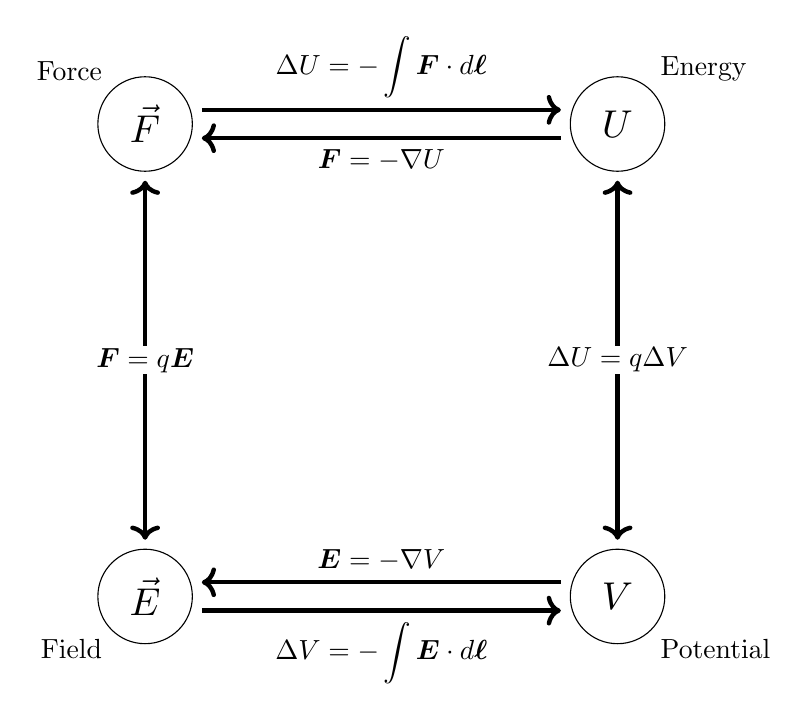
\begin{tikzpicture}[scale=0.6]
    % Nodes
    \draw[WHITE] (5,5) -- (5.707,5.707) node[black, anchor=south west] {Energy};
    \draw[BLACK] (5,5) circle (1);
    \node[BLACK] at (5,5) {$\displaystyle \Scale[1.4]{U}$};
    \draw[WHITE] (-5,5) -- (-5-0.707,5.707) node[black, anchor=south east] {Force};
    \draw[BLACK] (-5,5) circle (1);
    \node[BLACK] at (-5,5) {$\displaystyle \Scale[1.4]{\vec{F}}$};
    \draw[WHITE] (-5,-5) -- (-5.707,-5.707) node[black, anchor=north east] {Field};
    \draw[BLACK] (-5,-5) circle (1);
    \node[BLACK] at (-5,-5) {$\displaystyle \Scale[1.4]{\vec{E}}$};
    \draw[WHITE] (5,-5) -- (5.707,-5-0.707) node[black, anchor=north west] {Potential};
    \draw[BLACK] (5,-5) circle (1);
    \node[BLACK] at (5,-5) {$\displaystyle \Scale[1.4]{V}$};
    % Top Arrow
    \draw[BLACK, ultra thick, ->] (-3.8,5.3) -- (3.8,5.3) node[black, midway, above] {$\displaystyle \Delta U = -\int \bm{F} \cdot d\bm{\ell}$};
    \draw[BLACK, ultra thick, <-] (-3.8,4.7) -- (3.8,4.7) node[black, midway, below] {$\displaystyle \bm{F} = -\nabla U$};
    % Bottom arrow
    \draw[BLACK, ultra thick, ->] (-3.8,-5.3) -- (3.8,-5.3) node[black, midway, below] {$\displaystyle \Delta V = -\int \bm{E} \cdot d\bm{\ell}$};
    \draw[BLACK, ultra thick, <-] (-3.8,-4.7) -- (3.8,-4.7) node[black, midway, above] {$\displaystyle \bm{E} = -\nabla V$};
    % Right arrow
    \draw[BLACK, ultra thick, <-] (5,3.8) -- (5,0.3);
    \node[BLACK] at (5,0) {$\displaystyle \Delta U = q\Delta V$};
    \draw[BLACK, ultra thick, ->] (5,-0.3) -- (5,-3.8);
    % Left arrow
    \draw[BLACK, ultra thick, <-] (-5,3.8) -- (-5,0.3);
    \node[BLACK] at (-5,0) {$\displaystyle \bm{F} = q \bm{E}$};
    \draw[BLACK, ultra thick, ->] (-5,-0.3) -- (-5,-3.8);
\end{tikzpicture}
\label{fig:3:a}
\end{figure}

Everything thus far is from intro physics, so let's start adding some new stuff. We have both
\begin{equation*}
    \nabla \cdot \bm{E} = \frac{\rho}{\epsilon_o} \qquad \text{and} \qquad \bm{E} = -\nabla V.
\end{equation*}

Substituting the latter into the former yields
\begin{equation*}
    \nabla \cdot \underbrace{\left( -\nabla V \right)}_{\displaystyle \bm{E}} = \frac{\rho}{\epsilon_o} \quad \implies \quad \boxed{\nabla^2 V = -\frac{\rho}{\epsilon_o}}
\end{equation*}

which is Poisson's equation --- the partial differential equation that yields $V$ in electrostatics given a known source $\rho$.

\vspace{1em}

We will be solving Poisson's equation a lot in the near future, and to solve PDEs, we need boundary conditions. What might be the boundary conditions on $V$ be?

\vspace{1em}

Well, we know
\begin{equation*}
    \Delta V = V_{\text{above}} - V_{\text{below}} = -\int \bm{E} \cdot d\bm{\ell}
\end{equation*}

and real $\bm{E}$-fields are always finite. Thus, for sufficiently small $d\bm{\ell}$, $\displaystyle \Delta V \to 0$. In other words, as the path length shrinks to zero, so too does the integral:
\begin{equation*}
    V_{\text{above}} = V_{\text{below}} \qquad \boxed{\text{So } V \text{ is always continuous.}}
\end{equation*}

That being said, we know there can be discontinuities in $\bm{E}$. And $\bm{E}$-fields come about by taking derivatives of $V$ (recall that $\bm{E} = -\nabla V$). So consider some boundary, and let $n$ denote the direction normal to the boundary (pointing from ``below'' to ``above''). We have the boundary condition on the perpendicular component of the electric field:
\begin{equation*}
    E_{\text{above}}^{\perp} - E_{\text{below}}^{\perp} = \frac{\sigma}{\epsilon_o}
\end{equation*}

Using $\displaystyle E^{\perp} = -\frac{\partial V}{\partial n}$, gives us
\begin{equation*}
    \boxed{\frac{\partial V_{\text{below}}}{\partial n} - \frac{\partial V_{\text{above}}}{\partial n} = \frac{\sigma}{\epsilon_o}}
\end{equation*}

So while $V$ is always continuous, \emph{derivatives} of $V$ aren't necessarily. At least, not the derivative perpendicular to a boundary. Since $E^{\parallel}$ is continuous, so must be the derivative of $V$ in any direction parallel to the surface.

\begin{mdframed}[backgroundcolor=black!4, align=center, userdefinedwidth=0.8\textwidth, topline=false, bottomline = false, leftline = false, rightline = false, frametitle = {Interlude}]
\begin{center}
\iclicker[scale=0.28]Clicker question
\end{center}
\end{mdframed}

\vspace{1em}

\section*{Energy of a Charge Distribution}

What is the work it takes to move a charge $q$ from $\bm{x} = \bm{a}$ to $\bm{x} = \bm{b}$? We know work is given by $\displaystyle \int \bm{F} \cdot d\bm{\ell}$. The electric field exerts a force on the charge on the charge according to $\bm{F} = q\bm{E}$. Thus, the minimum force needed to overcome this field is $\bm{F} = -q\bm{E}$. It follows that the work done in moving a charge is
\begin{equation*}
    \text{Work } = \int \bm{F} \cdot d\bm{\ell} = -q \int_{\bm{a}}^{\bm{b}} \bm{E} \cdot d\bm{\ell} = q \left[ V(\bm{b}) - V(\bm{a}) \right].
\end{equation*}

Assuming we set the potential to be zero at infinity, the work required to bring in a charge from infinity to some location $\bm{x}$ is
\begin{equation*}
    \text{Work } = q \left[ V(\bm{x}) - \cancelto{0}{V(\infty)} \right] = q V(\bm{x}).
\end{equation*}

Imagine bringing a charge $q_1$ from infinity to the origin in empty space. This takes no work, since there is no field to fight against. However, once at the origin, the charge $q_1$ sets up a potential according to
\begin{equation*}
    V = \frac{1}{4\pi\epsilon_o} \frac{q_1}{\left| \bm{x} - \bm{x'} \right|} = \frac{1}{4\pi\epsilon_o} \frac{q_1}{r}.
\end{equation*}

The work done in bringing in another charge $q_2$ from infinity to some position $r$ is
\begin{equation*}
    W_{2} = q_2 \underbrace{\left( \frac{1}{4\pi\epsilon_o} \frac{q_1}{r} \right)}_{\displaystyle V} = \frac{1}{4\pi\epsilon_o} \frac{q_1 q_2}{r} \qquad\qquad \parbox[c]{0.4\textwidth}{This is the energy of interaction $U$ between two charges separated a distance $r$.}
\end{equation*}

Now we fix $q_1$ and $q_2$ in place, and let $r_{12}$ represent the distance between them. The work done in bringing in a third charge is
\begin{equation*}
    W_3 = q_3 \underbrace{\left( \frac{1}{4\pi\epsilon_o} \right) \left( \frac{q_1}{r_{13}} + \frac{q_2}{r_{23}} \right)}_{\displaystyle \text{potential from } q_1 \text{ and } q_2.}
\end{equation*}

\begin{figure}[H]
\captionsetup{width=0.8\textwidth, labelfont={color=black,bf}, textfont={color=black}}
\centering
\begin{tikzpicture}
    \filldraw[black] (0,0) circle (0.1) node[black, anchor=north west] {$q_1$};
    \draw[black, ->] (2,-1) .. controls (1.5,-1) and (0,-1) .. (0,-0.2);
    \draw[black] (0,0) -- (3,1) node[black, midway, anchor=north west] {$r_{13}$};
    \filldraw[black] (3,1) circle (0.1) node[black, anchor=north] {$q_3$};
    \draw[black, ->] (6,1) .. controls (5,1.25) and (3.5,0.75) .. (3.2,1);
    \draw[black] (3,1) -- (-2,2) node[black, midway, anchor=south west] {$r_{23}$};
    \draw[black] (0,0) -- (-2,2) node[black, midway, anchor=north east] {$r_{12}$};
    \filldraw[black] (-2,2) circle (0.1) node[black, above] {$q_2$};
    \draw[black, ->] (-5,1) .. controls (-4,2) and (-3,1) .. (-2.2,2);
\end{tikzpicture}
\label{fig:3:b}
\end{figure}

The total work in assembling these three charges is
\begin{equation*}
    W = \frac{1}{4\pi\epsilon_o} \left( \frac{q_1 q_2}{r_{12}} + \frac{q_1 q_3}{r_{13}} + \frac{q_2 q_3}{r_{23}} \right)
\end{equation*}

The work done in assembling a collection of discrete charges is also the energy we'd get if we dismantled the system. That is, it represents the energy stored in the configuration. We can generalize to $n$ number of particles:
\begin{equation*}
    U = \frac{1}{2} \left(\frac{1}{4\pi\epsilon_o}\right) \sum\limits_{i = 1}^{n} \sum\limits_{j \neq i}^{n} \frac{q_i q_j}{r_{ij}},
\end{equation*}

where the factor of $1/2$ arises because we're double counting each pair. Now, instead of a collection of discrete charges, consider some continuous charge distribution, with differential charge elements $dq_1$ and $dq_2$ (located on the same charge distribution). Then the sum becomes an integral and we have
\begin{equation}
    U = \frac{1}{2} \iint \frac{k\ dq_1\ dq_2}{r_{12}} = \frac{1}{2} \int \frac{k\ \rho(\bm{x}_1)\ \rho(\bm{x}_2)\ d^3x_1\ d^3x_2}{\left| \bm{x}_1 - \bm{x}_2 \right|} \tag{1} \label{eq:3:uu}
\end{equation}

Again, $\rho(\bm{x}_1)$ and $\rho(\bm{x}_2)$ describe the \underline{same} charge distribution --- we're breaking the charge distribution into little $dq$'s and check each against all the others.

\vspace{1em}

As an alternative, note that $\displaystyle \int \frac{k\ \rho(\bm{x}_1)\ d^3x_1}{\left| \bm{x}_1 - \bm{x}_2 \right|}$ is how we'd write the voltage due to $\rho$ at $\bm{x}_2$ (the location of the second charge in a particular pair). Thus, we can re-write the energy of the charge distribution as
\begin{equation}
    \boxed{U = \frac{1}{2} \int \rho(\bm{x'})\ V(\bm{x'})\ d^3x'} \tag{2} \label{eq:3:u}
\end{equation}

\begin{mdframed}[backgroundcolor=WHITE,align=left,userdefinedwidth=0.95\textwidth, topline=false, rightline=false,frametitle={Alternate derivation of (\ref{eq:3:u})}]

Start with the double sum that gives the energy of a collection of discrete charges:

\begin{equation*}
    U = \frac{1}{2} \left( \frac{1}{4\pi\epsilon_o} \right) \sum\limits_{i = 1}^{n} \sum\limits_{j \neq 1}^{n} \frac{q_i\ q_j}{r_{ij}}.
\end{equation*}

We can re-write this expression by pulling out a factor of $q_i$ from the second sum:

\begin{equation*}
    U = \frac{1}{2} \sum\limits_{i = 1}^{n} q_i \underbrace{\left( \sum\limits_{j \neq i}^{n} \frac{1}{4\pi\epsilon_o} \frac{q_j}{r_{ij}} \right)}_{\parbox[c]{0.14\textwidth}{\centering potential at $r_i$ (position of $q_i$) due to all other charges}} = \frac{1}{2} \sum\limits_{i = 1}^{n} q_i V
\end{equation*}

Now generalizing to a continuous charge distribution:

\begin{equation*}
    \boxed{U = \frac{1}{2} \int \rho (\bm{x'})\ V(\bm{x'})\ d^3x'}
\end{equation*}

\end{mdframed}

The expression for the energy of the system explicitly reference charge. This is not shocking --- we're used to potential energy being a thing associated with pairs of charges. But here's where it gets interesting. We're going to re-write the energy in terms of the field, thereby eliminating $\rho$ and $V$ in favor of $\bm{E}$.

\vspace{1em}

From Gauss's law, we know that $\displaystyle \nabla \cdot \bm{E} = \frac{\rho}{\epsilon_o} \implies \rho = \epsilon_o \left( \nabla \cdot \bm{E} \right).$. Substituting that into (\ref{eq:3:u}) gives us
\begin{equation*}
    U = \frac{\epsilon_o}{2} \int \left( \nabla \cdot \bm{E} \right)\ V\ d^3x.
\end{equation*}

For any scalar-valued function $f$ and vector-valued function $\bm{A}$, the following holds:
\begin{equation*}
    \nabla \cdot \left( f \bm{A} \right) = f \left( \nabla \cdot \bm{A} \right) + \bm{A} \cdot \left( \nabla f \right).
\end{equation*}

Taking $f = V$ and $\bm{A} = \bm{E}$, we have
\begin{equation*}
    \nabla \cdot \left( V \bm{E} \right) = V \left( \nabla \cdot \bm{E} \right) + \bm{E} \cdot \left( \nabla V \right) \implies \underbrace{\left( \nabla \cdot \bm{E} \right)\ V}_{\parbox[c]{0.088\textwidth}{\vspace{-0.28cm}\begin{center} \small matches integrand above \end{center}}} = \nabla \cdot \left( V\ \bm{E} \right) - \bm{E} \cdot \left( \nabla V \right)
\end{equation*}

Substituting, we get
\begin{align*}
    U &= -\frac{\epsilon_o}{2} \int \bm{E} \cdot \underbrace{\left( \nabla V \right)}_{\displaystyle -\bm{E}} d^3x + \frac{\epsilon_o}{2} \int \nabla \cdot \left( V\ \bm{E} \right)\ d^3x \\
    &= \frac{\epsilon_o}{2} \int \underbrace{\left( \bm{E} \cdot \bm{E} \right)}_{\displaystyle E^2}\ d^3x + \frac{\epsilon_o}{2} \int \nabla \cdot \left( V\ \bm{E} \right)\ d^3x
\end{align*}

Applying the divergence theorem to the second term yields
\begin{equation*}
    U = \frac{\epsilon_o}{2} \int E^2\ d^3x + \frac{\epsilon_o}{2} \oint \left( V\ \bm{E} \right) \cdot d\bm{A}
\end{equation*}

But what volume are we integrating over? Clearly, looking at the expression for energy in (\ref{eq:3:u}), we must at least integrate over the volume that encloses our charge distribution. But what's to stop us from integrating over all space? After all, $\rho = 0$ outside the charge distribution, so the extra space contributes nothing to the integral. Then the surface integral in the second term vanishes, since it examines $V$ and $\bm{E}$ at the edge of all space (which, for any real, finite source, is zero). Thus,
\begin{equation*}
    \boxed{U = \frac{\epsilon_o}{2} \int E^2\ d^3x} \qquad\qquad \parbox[c]{0.4\textwidth}{This is entirely in terms of fields, not charge. So we can look at the fields themselves as being very real things with real energy.}
\end{equation*}

Just for fun, let's take a look at the energy associated with the field made by a point charge at the origin. The field is
\begin{equation*}
    \bm{E} = \frac{1}{4\pi\epsilon_o} \frac{q\ \rhat}{r^2}
\end{equation*}

Substituting this into the energy expression and integrating over all space yields
\begin{align*}
    U &= \frac{\epsilon_o}{2} \int \bm{E} \cdot \bm{E}\ d^3x \\
    &= \frac{\epsilon_o}{2} \left( \frac{q}{4\pi\epsilon_o} \right)^2 \int \left( \frac{\rhat}{r^2} \cdot \frac{\rhat}{r^2} \right)\ d^3x.
\end{align*}

Note that $\rhat \cdot \rhat = 1$. Taking the differential volume element to be $r^2\ \sin{\theta}\ dr\ d\theta\ d\phi$, we get
\begin{align*}
    U &= \frac{\epsilon_o}{2} \left( \frac{q}{4\pi\epsilon_o} \right)^2 \int \frac{1}{r^4} r^2\ \sin{\theta}\ dr\ d\theta\ d\phi \\
    &= \frac{\epsilon_o}{2} \left( \frac{q}{4\pi\epsilon_o} \right)^2 \underbrace{\left( \int_0^{2\pi} d\phi \right)}_{\displaystyle 2\pi} \underbrace{\left( \int_0^{\pi} \sin{\theta}\ d\theta \right)}_{\displaystyle 2} \left( \int_0^{\infty} \frac{dr}{r^2} \right) \\
    &= \frac{q^2}{8\pi\epsilon_o} \int_0^{\infty} \frac{dr}{r^2} \\
    &= \frac{q^2}{8\pi\epsilon_o} \left( -\frac{1}{r} \right)\bigg|_{0}^{\infty} \qquad\qquad \text{which kind of diverges. That's bad.}
\end{align*}

What we just worked shows that $\bm{E}$-fields from point charges should contain infinite energy, thereby implying that point charges shouldn't be possible. But every experiment ever done indicates that an electron is a zero-radius true point. Fixing this apparent contradiction is one of the great achievements of quantum electrodynamics.

\section*{Delta Functions and Point Sources}

We've already seen indications that point charges behave a bit wonky, even though they do seem to exist experimentally. I'm afraid this is going to get a bit worse before it gets better.

\vspace{1em}

Let's take a look at Gauss's law again. If we take the divergence of an $\bm{E}$-field, we should recover the charge density that produced that field:
\begin{equation*}
    \nabla \cdot \bm{E} = \frac{\rho}{\epsilon_o}.
\end{equation*}

What happens if we take the divergence of the field made by a point charge at the origin? Applying the divergence operator in spherical coordinates gives us
\begin{equation*}
    \nabla \cdot \underbrace{\left( \frac{q}{4\pi\epsilon_o} \frac{\rhat}{r^2} \right)}_{\displaystyle \bm{E}_{\text{point}}} = \frac{1}{r^2} \frac{\partial}{\partial r} \left( \cancel{r^2} \frac{q}{4\pi\epsilon_o\ \cancel{r^2}} \right) = \frac{1}{r^2} \frac{\partial}{\partial r} \left( \frac{q}{4\pi\epsilon_o} \right) = 0\ \Scale[1.6]{?}
\end{equation*}

Well, according to that, the divergence of something like $\displaystyle \frac{\rhat}{r^2}$ is zero everywhere. Thus, so must $\rho$ be zero everywhere. But that can't be right. So what's the catch?

\vspace{1em}

The catch is that the operator $\displaystyle \frac{1}{r^2} \frac{\partial}{\partial r} \left( r^2 \right)$ isn't super well-defined at the origin. All we can conclude from the above is that $\nabla \cdot \bm{E}$ is zero everywhere \underline{but} the origin. To deal with the origin, let's take a look at delta functions first.

\vspace{1em}

A delta function is used to represent a finite amount of stuff compressed into an essentially zero-dimensional domain. In one dimension, a delta function $\delta(x)$ is \underline{defined} as the thingy that satisfies these two properties: $\delta(x)$ is a delta function if:

\begin{equation*}
    \displaystyle \delta(x) = \begin{cases} \displaystyle 0, & \text{if } x \neq 0 \\ \displaystyle \text{undefined}, & \text{if } x = 0 \end{cases}
\end{equation*}

and

\begin{equation*}
    \displaystyle \int \delta(x - a)\ f(x)\ dx = \begin{cases} \displaystyle f(a), & \text{if } a \text{ is in the domain of integration} \\ \displaystyle 0, & \text{otherwise} \end{cases}
\end{equation*}


Basically, it is a very sharply peaked function that, when present in an integral, plucks out the value of another function at one point:

\begin{figure}[H]
\centering
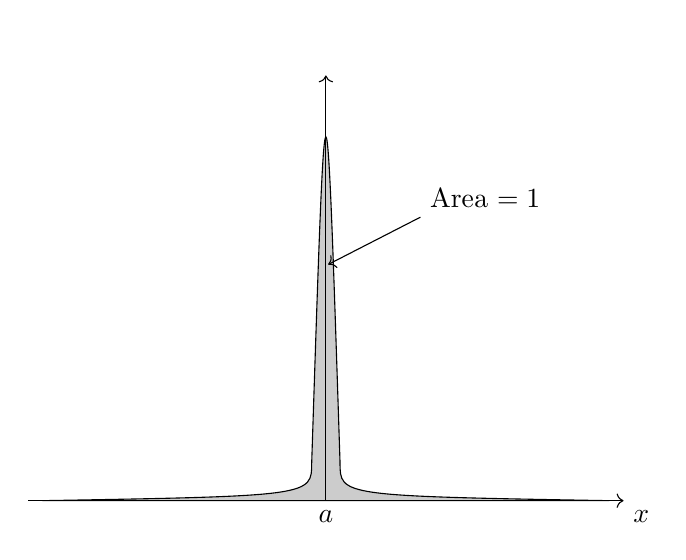
\begin{tikzpicture}[scale=0.6]
    \filldraw[color=black, fill=black!20] (-6,0) .. controls (-0.3,0.1) .. (-0.3,0.8) .. controls (0,10) .. (0.3,0.8) .. controls (0.3,0.1) .. (6,0) -- cycle;
    \draw[black, ->] (-6.3,0) -- (6.3,0) node[black, anchor=north west] {$x$};
    \draw[black, ->] (0,0) -- (0,9);
    \node[black, below] at (0,0) {$a$};
    \draw[black, <-] (0.05,5) -- (2,6) node[black, anchor=south west] {Area $= 1$};
\end{tikzpicture}
\label{fig:3:delta}
\end{figure}

So how do we represent $\rho$ for a point charge of size $q$ in 3D? How about a delta function:
\begin{equation*}
    \rho(\bm{x}) = q\ \delta^3(\bm{x}) \qquad\qquad \parbox[c]{0.33\textwidth}{(Or $\displaystyle q\ \delta^3(\bm{x} - \bm{x'})$ if the point charge is at $\bm{x'}$ instead of the origin)}
\end{equation*}

With that in mind, since $\displaystyle \nabla \cdot \bm{E} = \frac{\rho}{\epsilon_o}$, it should be the case that
\begin{equation*}
    \nabla \cdot \underbrace{\left( \frac{q}{4\pi\epsilon_o} \frac{\rhat}{r^2} \right)}_{\displaystyle \bm{E}_{\text{point}}} = \frac{1}{\epsilon_o} \underbrace{q\ \delta^3(\bm{x})}_{\displaystyle \rho}
\end{equation*}

And therefore
\begin{equation*}
    \nabla \cdot \left( \frac{\rhat}{r^2} \right) = 4\pi\delta^3(\bm{x}) \qquad\qquad \parbox[c]{0.25\textwidth}{Is this true?}
\end{equation*}

Well, it's true if
\begin{enumerate}

\item[(1)] $\displaystyle \nabla \cdot \left( \frac{\rhat}{r^2} \right) = 0$ everywhere but the origin. And we've established that.

\item[(2)] $\displaystyle \int \left( \nabla \cdot \frac{\rhat}{r^2} \right)\ d^3x = 4\pi$ for a domain of integration that includes the origin.

\end{enumerate}

Let's integrate $\displaystyle \nabla \cdot \left( \frac{\rhat}{r^2} \right)$ over a sphere of radius $R$. Just doing that as a volume integral is tricky, since the integrand is undefined at the origin, so let's dodge the bad part by using the divergence theorem:
\begin{align*}
    \int \left( \nabla \cdot \frac{\rhat}{r^2} \right)\ d^3x &= \oint \frac{\rhat}{r^2} \cdot d\bm{A} \\
    &= \oint \frac{\rhat}{r^2} \cdot \left( r^2\ \sin{\theta}\ d\theta\ d\phi\ \rhat \right) \\
    &= \oint \sin{\theta}\ d\theta\ d\phi \\
    &= \underbrace{\left( \int_0^{\pi} \sin{\theta}\ d\theta \right) \left( \int_0^{2\pi} d\phi \right)}_{\displaystyle =\ 4\pi}
\end{align*}

So it checks out. $\displaystyle \nabla \cdot \left( \frac{\rhat}{r^2} \right) = 4\pi\ \delta^3(r)$, and then
\begin{equation*}
    \nabla \cdot \left( \frac{q}{4\pi\epsilon_o} \frac{\rhat}{r^2} \right) = \frac{1}{\epsilon_o} q\ \delta^3(r) = \frac{\rho}{\epsilon_o}
\end{equation*}

and Gauss's law holds.

\end{document}
